
  
  

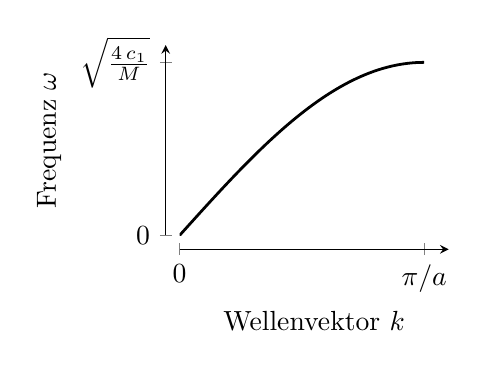
\begin{tikzpicture}[
declare function={ 
	  },
]
%\useasboundingbox (0,0) rectangle (5,5);
%\draw (0,0) rectangle (5,5);

\begin{axis}[no markers, 
	samples=150,
    %      ymin=-0.3, ymax=1,
      xmin = 0., xmax = 1.1,
    ymin = 0, ymax = 1.1,
      %  axis y line=left,
       %    axis x line=bottom,
          xtick = {0,1},
          xticklabels= {0, $\pi/a$},
      %     xticklabels = {\footnotesize $R_g$, \footnotesize $R_e$},
        %   ytick = {0,0.5, ..., 5.5},
         %  yticklabels = { , $1/2$, , $3/2$, , $5/2$, , $7/2$, , $9/2$, , $11/2$},
        ytick = {0,1},
           yticklabels = { 0, $ \sqrt{\frac{4 \, c_1}{M}}$},
            xlabel = {Wellenvektor $k$ },
        ylabel = {Frequenz $\omega$},    
        %x label style={at={(axis description cs:1, 0)},anchor=north east, yshift=-7pt},
    %y label style={at={(axis description cs: 0,1)},anchor=south east,  yshift=10pt},
           width= 5cm, height = 4cm,
  separate axis lines,
  axis x line=bottom,
  axis x line shift=5pt,
  %xlabel shift=10pt,
  axis y line=left,
  axis y line shift=5pt,
%  ylabel shift=10pt           
           ]
           
\addplot [domain=0:1,  line width=1pt]    {abs(sin(x * 90))};
 
%\foreach \a in {0,...,3}
%{
%  		\tikzmath{\b = E(\a); }          
%         % \addplot[gray] coordinates   {(-5,\b )  (5,\b)} ;
%       \addplot [smooth, fill=gray, domain=-3.5:3.5,  line width=0pt]    {E(\a) + 5 * (H\a(xi(x)) * decay(xi(x)) )^2 };
%}
%
%\tikzmath{\dr = 1; \de=4.5; }      
%\addplot [domain=-3.5:1.5,  line width=1pt]    {U(x+\dr) - \de};
%  \addplot [smooth, fill=gray, domain=-3.5:1.5,  line width=0pt]   
%   {E(0) - \de + 5 * (H0(xi(x + \dr)) * decay(xi(x + \dr)) )^2 };
%   
%\node[anchor = north, yshift=1mm] at (1.5, -1 * \de + 0.5) {\footnotesize $\nu = 0$} ;
%\node[anchor = north, yshift=1mm] at (3,  0.5) {\footnotesize $\nu = 0$} ;
%\node[anchor = north, yshift=1mm] at (3,  1.5) {\footnotesize $\nu = 1$} ;
%\node[anchor = north, yshift=1mm] at (3,  2.5) {\footnotesize $\nu = 2$} ;
%
%\draw [->] (-0.8,-1 *\de + 0.5) --  (-0.8, 0.5);
%\draw [->] (-1,-1 *\de + 0.5) --  (-1, 1.5);
%\draw [->] (-1.2,-1 *\de + 0.5) --  (-1.2, 2.5);
%
%\node[anchor = north, yshift=1mm] at (1.5,  -2) {\footnotesize $g$} ;
%\node[anchor = north, yshift=1mm] at (0.5,  0) {\footnotesize $e$} ;


 \end{axis}

\end{tikzpicture}


